\graphicspath{{Images/}}

\section{Introduction}
\subsection{It's an information revolution}
Information is everything. Information is ubiquitous. Information is a name, an email address, an IP address (a digital address), where you live (a physical address), a place of employment, a birthday, a file, a password, a text message, a credit card number, votes in an election, military deployment plans, and more. Information is created everyday, and it is exchanged everyday. It is interwoven with, provides guidelines for, and supports fields and domains that are simultaneously specific and private, owned and affected by the collective, as well as broadly applicable. Information science is a well-established field, and records proving its existence go as far back as the Library of Mesopotamia \cite{30s_history_of_info_science} even though the area of study did not receive its official name until about 1955 \cite{wiki_info_science}. Alan Turing sought to define information science as a ``universal, hardware-independent notion of computation"; whereas, Claude Shannon sought to define information science as a ``universal, meaning-independent notion of communication". Oxford Languages defines \textbf{\gls{info_sci}} as:
    \begin{quote}
        ``a broad and interdisciplinary field that studies how information is created, collected, organized, stored, retrieved, and used by humans and machines. It also examines the social, ethical, legal, and cultural aspects of information and its impact on society." \cite{bing_is_def}
    \end{quote}

\begin{figure}[ht] 
    \centering
    \ffigbox[\FBwidth]
        {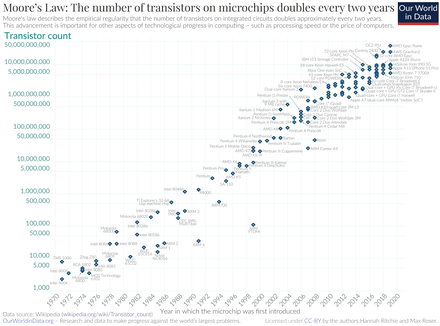
\includegraphics[width=0.65\textwidth]{moores_law.png}}
        {
            \captionsetup{justification=centering}
            \caption{Moore's law is the observation and subsequent prediction the number of transistors per microchip will double every two years}
            \label{fig:moores_law}
        }
\end{figure}

The \textbf{\gls{info_rev}} brought about by the advent of computers and the speed of its growth is quickly summarized using \textbf{\gls{moore}}. Originally published in Electronics Magazine in 1965, Gordon Moore predicted ``the number of transistors per square inch on a microchip would double each year while the manufacturing cost per component would halve" \cite{arcuri_moores}. This was revised a decade later to state ``chip density would...double every two years for at least the next decade
" \cite{arcuri_moores}.

Up until now, Moore's law has quite faithfully remained true, much to Moore's own surprise, made possible because engineers were able to continually develop smaller and smaller transistors. Well-known and regarded as a general rule rather than just a theorem in information science, its veracity has exceeded the predicted ten-year lifetime by more than thirty years as illustrated in Figure \ref{fig:moores_law}, but all good things must come to an end. As of 2016, the smallest transistor yet is roughly the same thickness as a single layer of carbon atoms \cite{yang_transistor}. Sarah Yang from the Berkeley National Lab remarked in ``Smallest transistor ever made by Berkeley Lab" that transistors reaching the atomic scale may be the end of Moore's law as we know it, but maybe the end of one chapter is just the beginning of another. 

\subsection{Time for a quantum revolution: The future is... now?} \label{q_rev}
The study of quantum mechanics goes all the way back to the early 1800s \cite{q_mech_timeline}. Essentially the physics of small things \cite{qc_explained}, the field of quantum mechanics paved the way for the field of quantum computing. When Stephen Wiesner invented conjugate coding in 1965 \cite{qc_timeline}, this marked the beginning of quantum communication and computation and, arguably, a brand new information revolution. Whereas the invention of the classical computer spurred on the growth of the field of information science and provided the foundation for areas of study such as classical communication, computation, and cryptography, the invention of the quantum computer (\textbf{\gls{qc}}) has great promise to do the same.

In an article as recent as October 2023, a quantum computer boasting a record-breaking 1,180 qubits was build by tech startup Atom Computing \cite{atom_computing}. This broke IBM's standing record with their quantum computer, Osprey, having a, what now seems small, 433 qubits (as recent as 2022) \cite{osprey}. In a vein that seems vaguely familiar to Moore's law, this innovation is notable not only because it represents a rapid level of innovation in an unexpectedly short amount of time, this recent news may indicate that quantum computing has the power to usher in new eras of quantum communication, computation, and cryptography in much the same fashion that classical computers kick-started the information revolution beginning in the early 1980s. With quantum computers promising to be more powerful and better at solving complex problems, increased power means great potential to be used for good or bad. 

As an example, Shor's 1994 algorithm promises to be able to effectively do prime factorization with ``strong evidence of super-polynomial speedup" \cite{wiki_shor}. This is significant because the security of many public-key protocols is built on the premise that multiplying two primes is very easy, but given the their product, it is difficult to find it's prime factors especially if these primes were very large. In general, an ideal property for any cryptography scheme to have is that is it easy to compute but difficult to reverse unless you know a secret piece of information, and Shor's algorithm tells us that, backed by the power of quantum computers, public-key protocols used every day by individuals, companies, and world governments for encrypting sensitive and critical data as well as providing digital signatures may be at risk of being broken, leaving the information they protect vulnerable to stealing and exploitation.

\begin{figure}[h] \centering
    \ffigbox[\FBwidth]
        {
            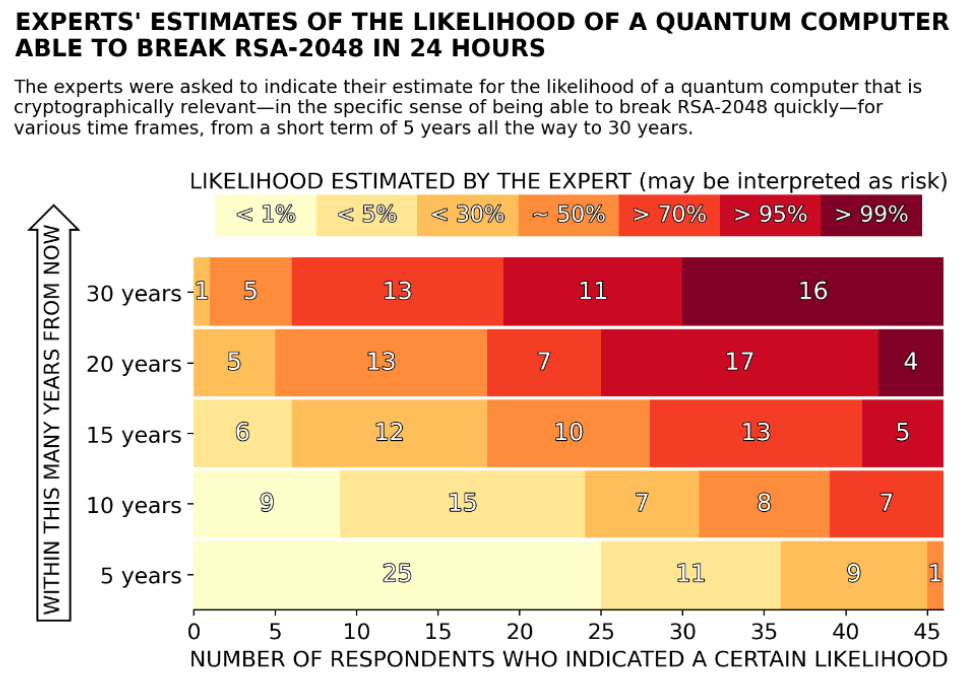
\includegraphics[width=.47\textwidth]{mosca_piani.png}
            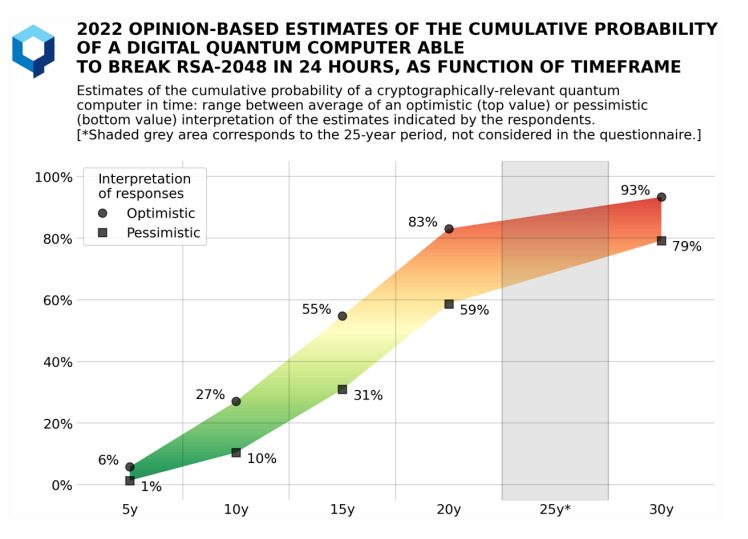
\includegraphics[width=.47\textwidth]{crqc22.png}
        }
        {
            \captionsetup{justification=centering}
            \caption{Mosca and Piani's 2022 survey shows estimates for when a cryptographically-relevant quantum computer may be made range from 5 to 30 years} \label{fig:mosca_piani}
        }
\end{figure}

We have already seen evidence that the quantum field is growing at a rapid pace to say the least. The threat this poses to the current security infrastructure as we illustrated is palpable. If recent developments are any indicator of where the field is going and the cadence it will maintain going forward, it is essential that developments on the defensive security side are worked concurrently, and they must try to keep pace. So far it seems that cryptographers are up to the challenge, and several exciting and interesting discoveries have come out as a byproduct of this work and research. The only question left weighing on many people minds is ``how much time do we have?" which snowballs into other questions such as ``do we have enough time?", ``what can we reasonably expect to accomplish in the time we have?", and ``if we don't have time to do everything we want, what should we prioritize?".

These very questions have received a certain amount of research of their own. Something that may cause anxiety due to the uncertainty of it all or may provide some relief is that computers capable of such computations do not yet exist; however, different researchers have tried to predict when such a computer could be expected, but have come up with answers that range from 5 to 30 years (Figure \ref{fig:mosca_piani}) \cite{mosca_piani_howsoon}. Meanwhile, the US government believes that ``adversarial nation-states are currently investing billions of dollars to weaponize quantum computers" \cite{2022_nsa}. In other words, we aren't entirely sure, but doesn't mean we're clueless. 

\textbf{\gls{moscas_theorem}}, named after renowned mathematician and computer scientist Michele Mosca, gives us a formula by which to judge such questions. More specifically it gives us a formula for us to judge how long we have to find a quantum-safe, -resistant, or -resilient solution and implement it before critical information and systems will be at risk (Figure \ref{fig:moscas_theorem}). \\

    \begin{table}[h]
        \centering
        \begin{tabular}{cl}
     \multicolumn{2}{c}{Given:}\\
             $x \leftarrow$& shelf-life time or how long we need encryption to be secure\\
             $z \leftarrow$& threat timeline or time until large-scale quantum computer is built\\
        \end{tabular}
        \label{tab:mosca_given}
    \end{table}
    
    \begin{table}[h]
        \centering
        \begin{tabular}{cl}
     \multicolumn{2}{c}{We have:}\\
             $y \leftarrow$& migration time or time we have to find a quantum-safe solution and retool existing architecture\\
        \end{tabular}
        \label{tab:mosca_wehave}
    \end{table}
    
    \begin{table}[h]
        \centering
        \begin{tabular}{cl}
     \multicolumn{2}{c}{Which tells us:}\\
             \multicolumn{2}{c}{If $x+y>z$, then it's time to worry!}\\
 \multicolumn{2}{c}{So we need to make sure $y < z-x$}\\
        \end{tabular}
        \label{tab:mosca_worry}
    \end{table}
    
    \begin{figure}[!h]
        \centering
        \ffigbox[\FBwidth]
        {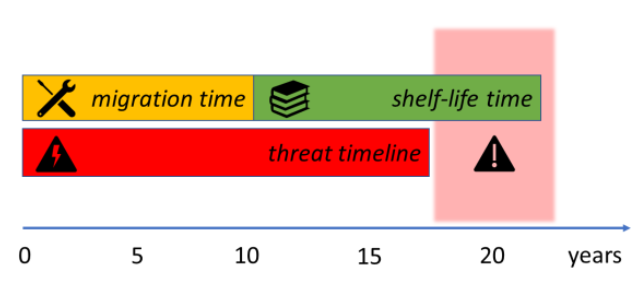
\includegraphics[width=0.65\linewidth]{moscas_theorem.png}}
        {
            \captionsetup{justification=centering}
            \caption{Mosca's theorem gives a mathematical method for conceptualizing the amount of time before quantum resistant/resilient cryptography will be necessary}
            \label{fig:moscas_theorem}
        }
    \end{figure}
    
Mosca's theorem goes hand in hand with a concept becoming increasingly well-known and referenced called a catch-and-exploit attack. In ``Preparing Critical Infrastructure for Post-Quantum Cryptography" written and released by the Cybersecurity and Infrastructure Security Agency \textbf{\gls{cisa}} (an operational component of DHS), a catch-and-exploit campaign is defined as an attack in which ``adversaries capture data that has been encrypted using current encryption algorithms and hold onto such data with the intention of decrypting it when a quantum computer capable of breaking the encryption is available" \cite{cisa_prep4pqc}. This concept is important because it indicates the possibility that once a cryptographically-relevant quantum computer (\textbf{\gls{crqc}}) is made and available data assets may be at risk almost immediately, and it emphasizes the importance of updating the systems that protect and transmit this data as soon as possible. 

The stakes are high, and it is under these circumstances that the US government has banded together to find a solution. While the National Security Agency (\textbf{\gls{nsa}}) searches for possible solutions to protect US National Security Systems (\textbf{\gls{nss}}), the National Institute for Science and Technology (\textbf{\gls{nist}}) has been given the task finding, vetting, and standardizing quantum-safe protocols that could be used to phase out and replace systems currently in use that are most likely to be broken first once quantum computers are widely available. Meanwhile, the Department of Homeland Security (\textbf{\gls{dhs}}) has been tasked with writing and disseminating recommendations for other public sector organizations (\textbf{\gls{fceb}} agencies, \textbf{\gls{sltt}} government organizations) and private sector organizations that provide any of the National Critical Functions (\textbf{\gls{ncf}}s) or support the critical infrastructure (\textbf{\gls{ci}}). 

\subsection{Cryptography in a Post-Quantum World} 
In this paper, we will discuss how the world of cryptography may be affected by the invention and development of quantum computers. This is an introductory discussion; therefore, we will aim to explain broad concepts using simple language. As such, the discussion will not be overly technical, but there are vast resources online which discuss the underlying implementation details, mechanics, and more taught by a variety of individual and organizations ranging from hobbyists to the inventors themselves. We will begin with an explanation of some background topics (Section \ref{quantum_basics}) important to understanding the benefits and limitations of quantum computers. We will then discuss how these basic concepts backed the invention of some foundational systems in quantum cryptography (Section \ref{q_crypto}). We will briefly explain Shor's Algorithm and Grover's Algorithm to understand what they are, why they are important, and how they affect current work in the cryptographic field (Section \ref{shor_grover}). To provide a broad picture of how such work is affecting significant change in our world, we will talk about how the NSA, NIST, and DHS have been working together to secure our future (Section \ref{government}). Post-quantum cryptography standardization is an area of research still very much alive, and there is no better illustration of this than NIST's Post-Quantum Cryptography (\textbf{\gls{pqc}}) Standardization Competition which we will close with in order to give readers the latest update of where the world stands in this development process, what we currently know, and where we predict it will head next (Section \ref{industry}). This discussion will go back and forth between the conceptual and the tangible, leaning more and more heavily on the tangible side of things as we progress. As the discussion becomes more and more tangible and of the moment, we will try to use more and more real life examples to illustrate concepts while remaining introductory friendly. With that, it should be noted that this report cannot with any level of certainty know for sure where and how this industry and this process will conclude or when. We have sourced as many sources as possible within the given time frame to paint a picture of the work and how it currently stands as of the time of writing for the reader. It is our hope is that this paper will provide a good foundation, arming the reader with the knowledge base necessary follow this movement after the writing of this paper, past the initial stages of standardization, and into the growth of the wider industry. Thank you for taking the time, and welcome to the quantum revolution. 

% \redcomm{Hello}
% \greencomm{Hello 2}
% \bluecomm{Hello 3}

% \gls, \Gls, \glspl, \Glspl

